\documentclass{article}
\usepackage[T1]{fontenc}
\usepackage{lmodern}
\usepackage{graphicx}
\usepackage{amsmath,amssymb}
\usepackage[a4paper,margin=2cm]{geometry}
\usepackage[absolute,overlay]{textpos}
\setlength{\TPHorizModule}{1mm}
\setlength{\TPVertModule}{1mm}
\usepackage[indonesian]{babel}
\usepackage{hyperref}
\setlength{\emergencystretch}{2em}
% unit: Halaman 20

\begin{document}

% === Halaman 20 (llm) ===

\vspace{286.31mm}

\section*{Kebocoran data penguna Tokopedia}

\vspace{10mm}

\vspace{10mm}

% deskripsi: Screenshot cuitan Twitter dari akun Under the Breach yang menginformasikan kebocoran database Tokopedia pada Maret 2020, lengkap dengan cuplikan data yang bocor.
% bbox normalisasi: [0.0970, 0.1830, 0.5410, 0.8860]
\begin{textblock*}{93.24mm}(20.37mm,54.35mm)
\noindent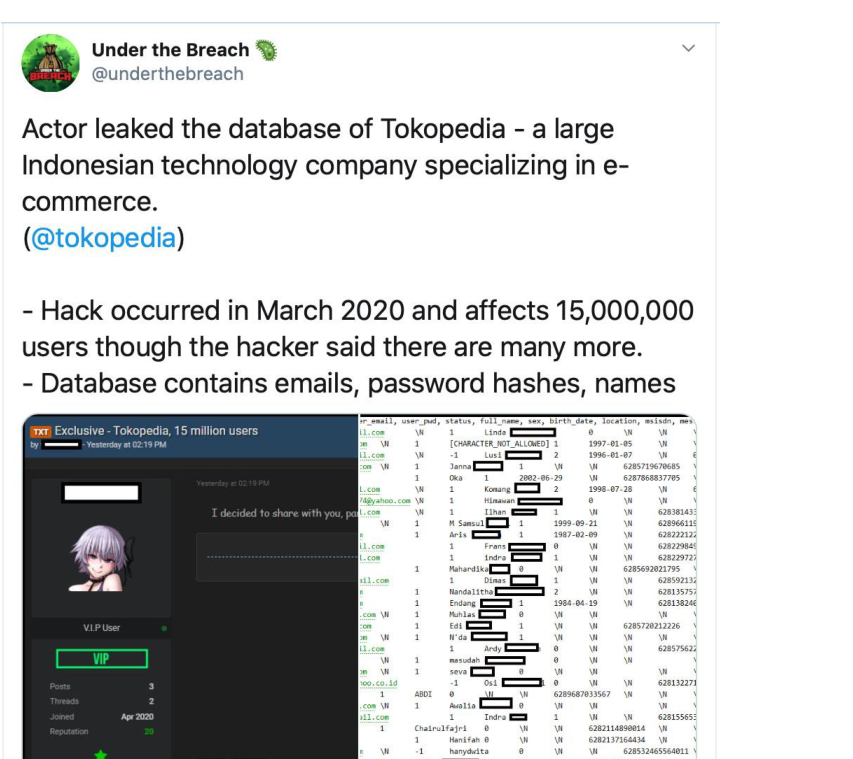
\includegraphics[width=93.24mm,height=208.79mm]{../../images/llm/page_020_img_01.png}%
\end{textblock*}

% deskripsi: Infografis dari Katadata mengenai pencurian data di e-commerce, merinci kebocoran data Tokopedia (2020) dan Bukalapak (2019) termasuk jumlah data dan harga jualnya.
% bbox normalisasi: [0.6100, 0.0000, 0.9030, 0.9640]
\begin{textblock*}{61.53mm}(128.10mm,0.00mm)
\noindent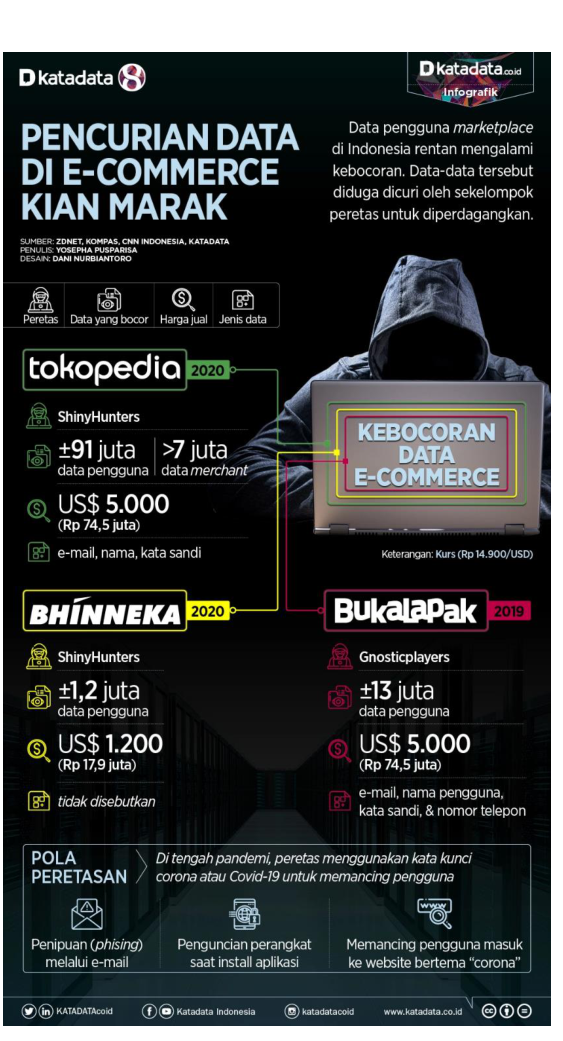
\includegraphics[width=61.53mm,height=286.31mm]{../../images/llm/page_020_img_02.png}%
\end{textblock*}

\end{document}
